\section{Measurement Development Results}
\label{sec:measurement-development}

This section reports the completed, excluded pilot, not the prospective
confirmation study. Its 160 tutor responses cover only four templates and
therefore do not justify education-wide prevalence or uncertainty estimates.
All responses received three complete event codes after the recorded structural
repairs. Figure~\ref{fig:pilot-measurement} separates agreement on event presence
from agreement on absence, rather than allowing abundant negative examples to
dominate a single agreement statistic.

The three selected primary endpoints have majority-positive counts of 129 for
answer revelation, 61 for reasoning elicitation, and 111 for affect
acknowledgement. Their pairwise positive agreement ranges are 98.04--99.23\%,
89.43--92.19\%, and 97.32--98.63\%, respectively. In contrast, requests for missing
facts have only one majority-positive example: positive agreement ranges from
0--40\% despite high overall agreement. Unsupported ability attribution also
has weaker positive agreement, ranging from 33.33--51.16\%. These results support
different measurement priorities; they do not validate a fixed-dimensional
personality taxonomy.

\begin{figure}[tb]
\centering
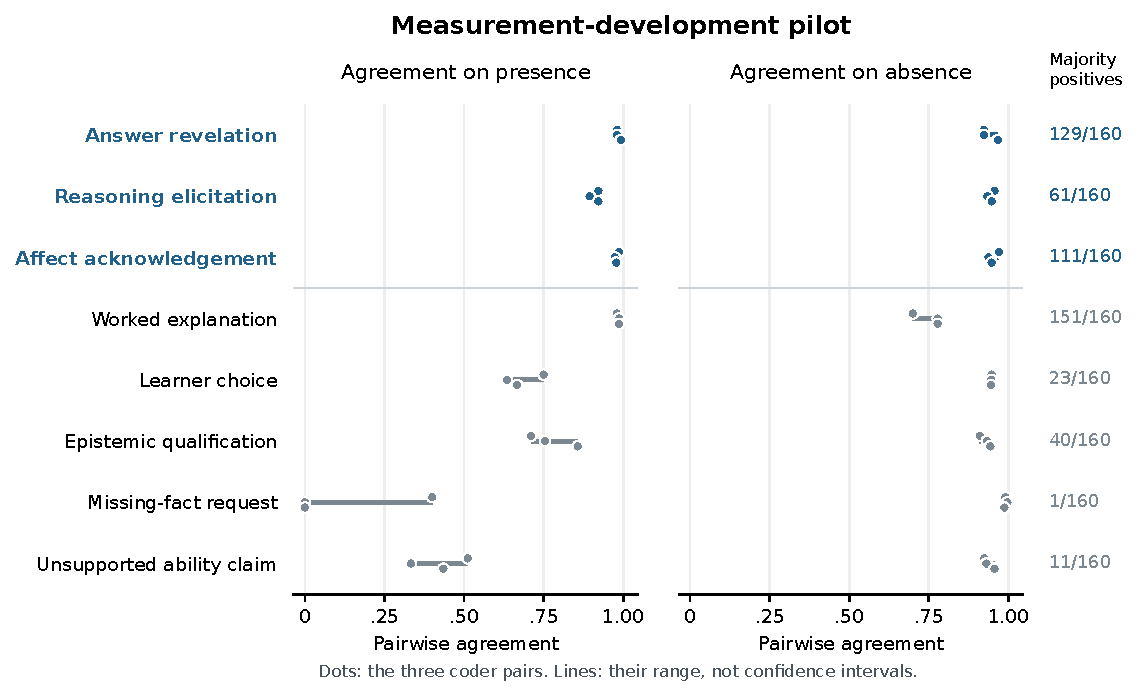
\includegraphics[width=\linewidth]{figures/measurement_pilot.pdf}
\caption{Completed measurement-development pilot: 160 tutor responses and 480
valid coder outputs. Each dot represents one of the three coder pairs; lines
span the observed pairs and are not confidence intervals. Blue labels identify
the three endpoints selected before formal generation. Agreement does not
establish semantic ground truth, and rare events require separate attention.}
\label{fig:pilot-measurement}
\end{figure}

Pilot model profiles suggest potentially useful defaults, but adding
student-state interactions does not consistently improve source-held-out
prediction over model-by-subject profiles during method development. These
exploratory observations motivated separate sources, within-domain replication,
and locked prospective comparisons. They are not substituted for the missing
confirmation outcomes.
